\section[Design Strategy]{Design Strategy on Embedded (Real-time) Software}
\subsection{Targets}
\begin{itemize}
	\item Design should be solution independent for as long as it makes sense (not as long as possible).
	\item Encourage system design, rather than separate designs for mechanics, electronics, firmware, software, etc., which may be conflicting
	\item System specification is ideally done using a unique specification language, not in prose
	\item The specification can be simulated (executed)
	\item Implementations can be easily changed, e.g. from HW to SW or vice versa.
\end{itemize}

\subsection{Requirements for Practical Application}
\begin{itemize}
	\item Methods and tools should not be too technical in system design, i.e. methods should be applicable for electronics, firmware and if possible also mechanics developers
	\item If possible good tool support and automatic synthesis
\end{itemize}

\subsection{Specification Languages}
\begin{itemize}
	\item Formal languages are unique
	\item Examples of specification languages: SystemC, SysML, SpecC, SystemVerilog, Esterel, Matlab/Simulink, Statecharts.
	\item The specification can be compiled and executed
	\item Simulations of the system on a powerful system (e.g. PC) are mostly supported
	\item The executable specification serves as golden reference for future development steps
\end{itemize}

\subsection{Approach}
Approach in a real time embedded design for task and scheduling topics
\begin{enumerate}
	\item Analysis of requirements and split work up into tasks
	\item The system and task model
	\item The scheduling algorithm with related schedule ability test.
	      Implement every flow and measure WCET.
	\item Theoretical and/or empirical performance evaluation of the scheduling algorithm and/or the schedule ability test
\end{enumerate}

\subsubsection{Split Work up into Tasks}
Get the system's timing constraints from \ldots
\begin{itemize}[label=\ldots]
	\item the physics of the system and their implications
	\item the application
\end{itemize}
Data flow charts help to split ub data paths into tasks.

\subsubsection{Classify Tasks}
\begin{minipage}[b]{0.6\textwidth}
	First task of a system architect is to classify the tasks into the structure like below.
	Every task of a lower class can be implemented in a higher class.
	A task without timing constraints mostly does not exist, however for the sake of completness it is arranged and shown here.
	Strict periodic and event driven tasks are similar in their priority since they are both implemented in ISR.
\end{minipage}
\begin{minipage}{0.39\textwidth}
	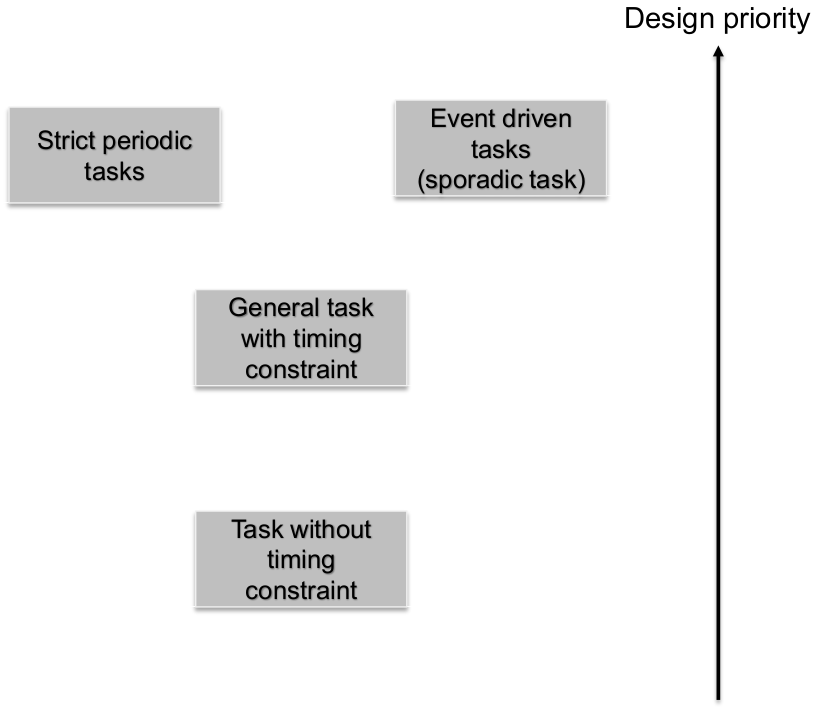
\includegraphics[width=\textwidth]{images/DesignStrategy/classify_tasks.png}
\end{minipage}


\subsubsection{Implementation without RTOS}
% \begin{minipage}[b]{0.6\textwidth}
The classification leads to the implementation in three different areas: Timer-ISR, ISR and main.
First steps can and should be implemented and tested separately.
Especially to determine WCET.
Since the ISR influence each other, tests must be undertaken with both implementations.
Last Step is to test the whole software architecture concerning real time behavior.

% \end{minipage}
% \begin{minipage}{0.39\textwidth}
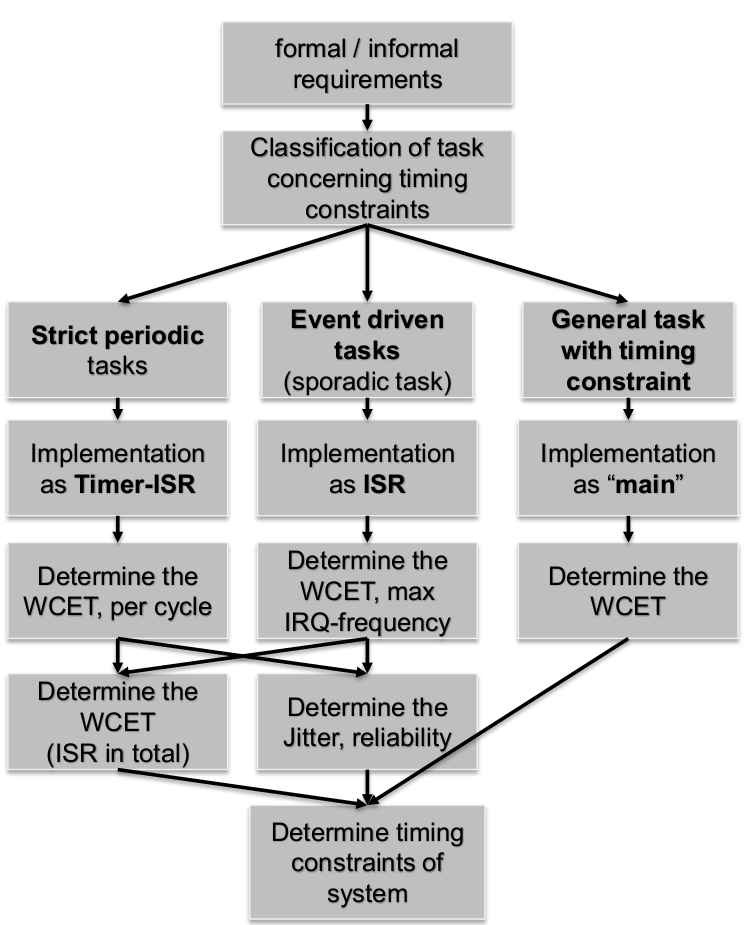
\includegraphics[width=0.4\textwidth]{images/DesignStrategy/task_implement_no_rtos.png}
% \end{minipage}

\subsubsection{Implementation with RTOS}
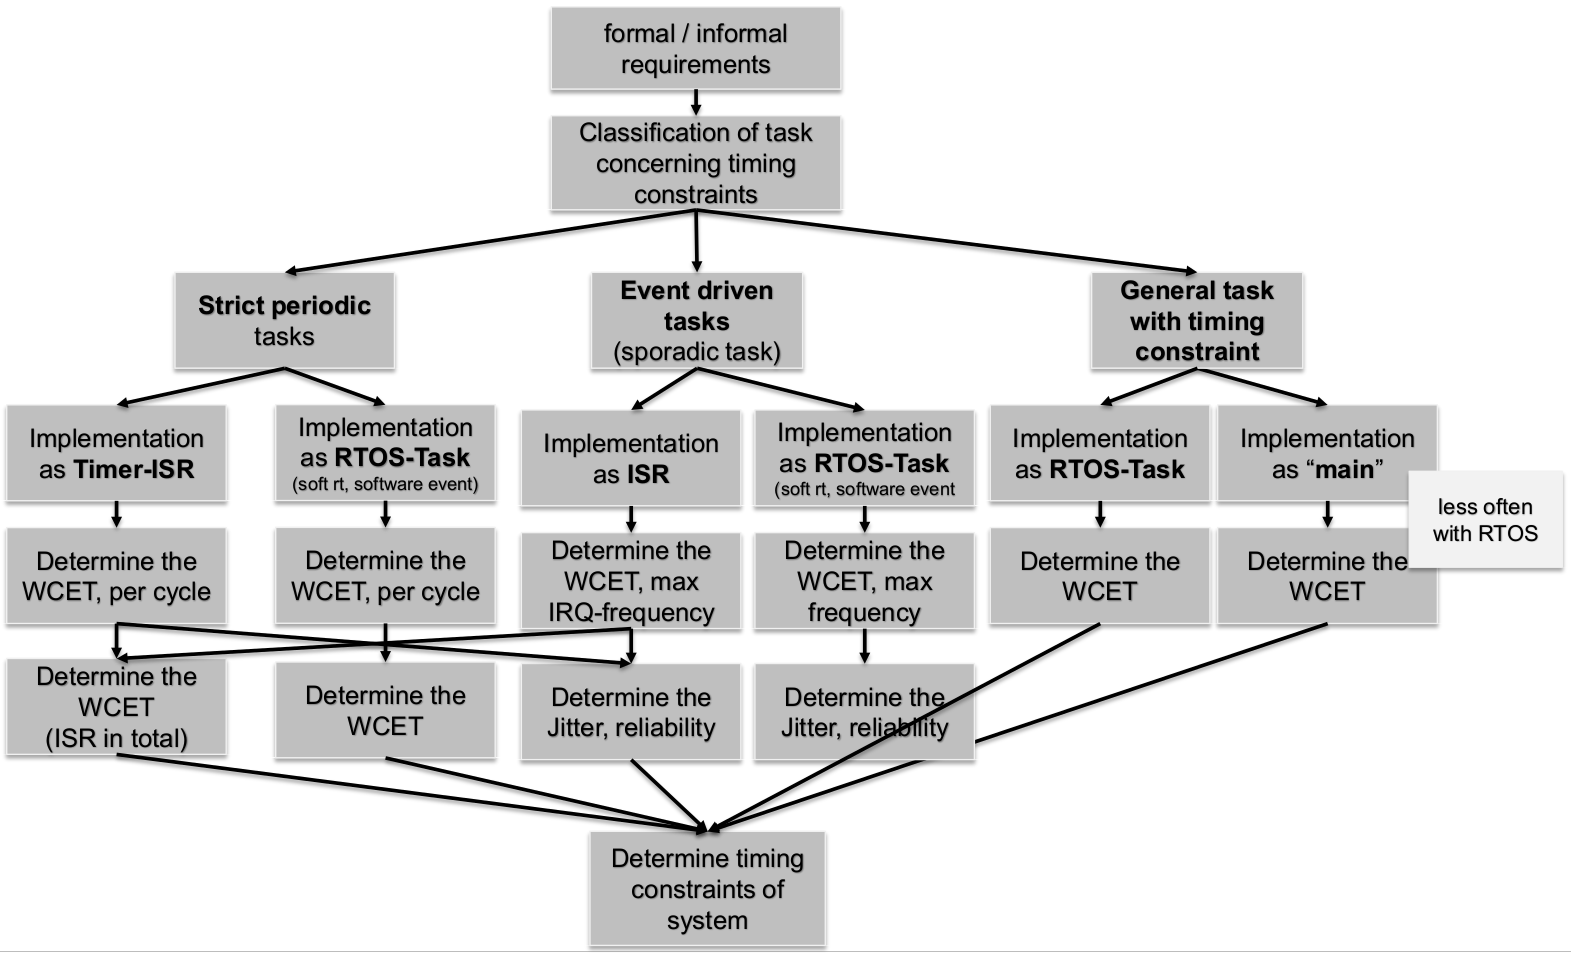
\includegraphics[width=0.9\textwidth]{images/DesignStrategy/task_implement_rtos.png}

\subsection{Approaches to define static Priorities for Tasks}
\subsubsection{Rate-Monotonic Approach: Short Code High priority}
The idea is that short ISR/tasks are executed fast.
Therefore, they block fo a very short time and execution is more guaranteed by priority.
\begin{itemize}
	\item Shortest ISR has highest priority
	\item Shortest flow/task has highest priority
\end{itemize}

\subsubsection{Important Code High Priority}
The idea is important ISR/tasks are executed fast.
\begin{itemize}
	\item Important ISR has highest priority
	\item Important task has highest priority
\end{itemize}

\subsubsection{Blended Approach}
Combination of RMA and ICH
\begin{itemize}
	\item Short task high priority
	\item Important ISR has high priority
\end{itemize}

\subsection{Interrupt Handling Concepts}
There are two main concepts how interrupt handling is implemented.

\begin{table}[h]
	\begin{tabularx}{\textwidth}{lXX}\hline
		Name        & Service Routine (ISR)                            & RTOS Task                                          \\\hline
		Description & Event code is executed mainly in the ISR         & ISR passes every executing code to RTOS task       \\
		Pros        & - Fastest execution                              & - RTOS support\newline - Interrupts fast available \\
		Cons        & - No or small RTOS support\newline - Blocks RTOS & - Slower execution, depended on RTOS scheduling    \\\hline
	\end{tabularx}
\end{table}

The approach of: \textbf{Interrupt handler in the RTOS task} is also called \textbf{software events} approach.
In a project they can also be combined.

\subsection{Prioritizing Interrupts, RTOS and Handling}
The real time system architecture can be influenced by defining the priority of the system timer of the RTOS!
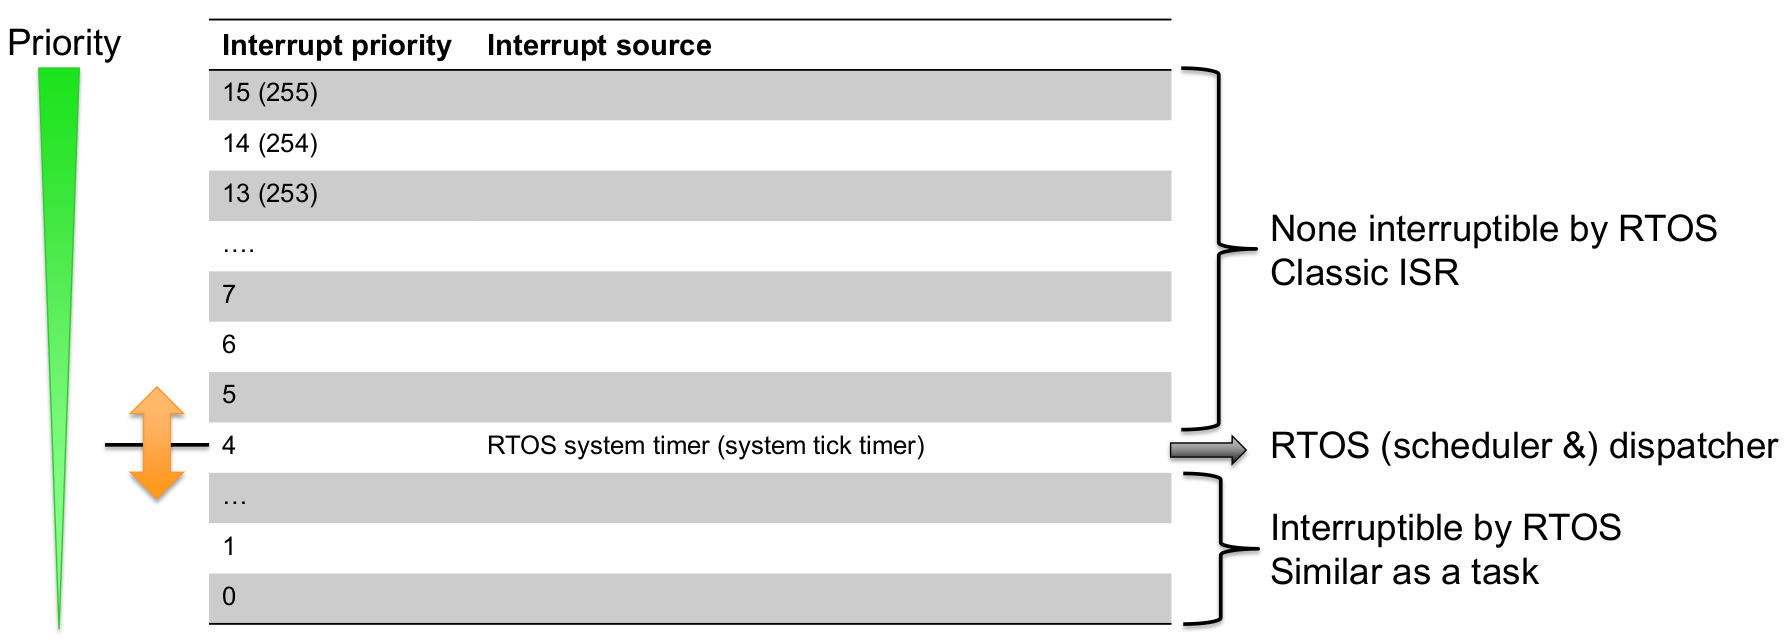
\includegraphics[width=\textwidth]{images/DesignStrategy/prio_interrupts.png}
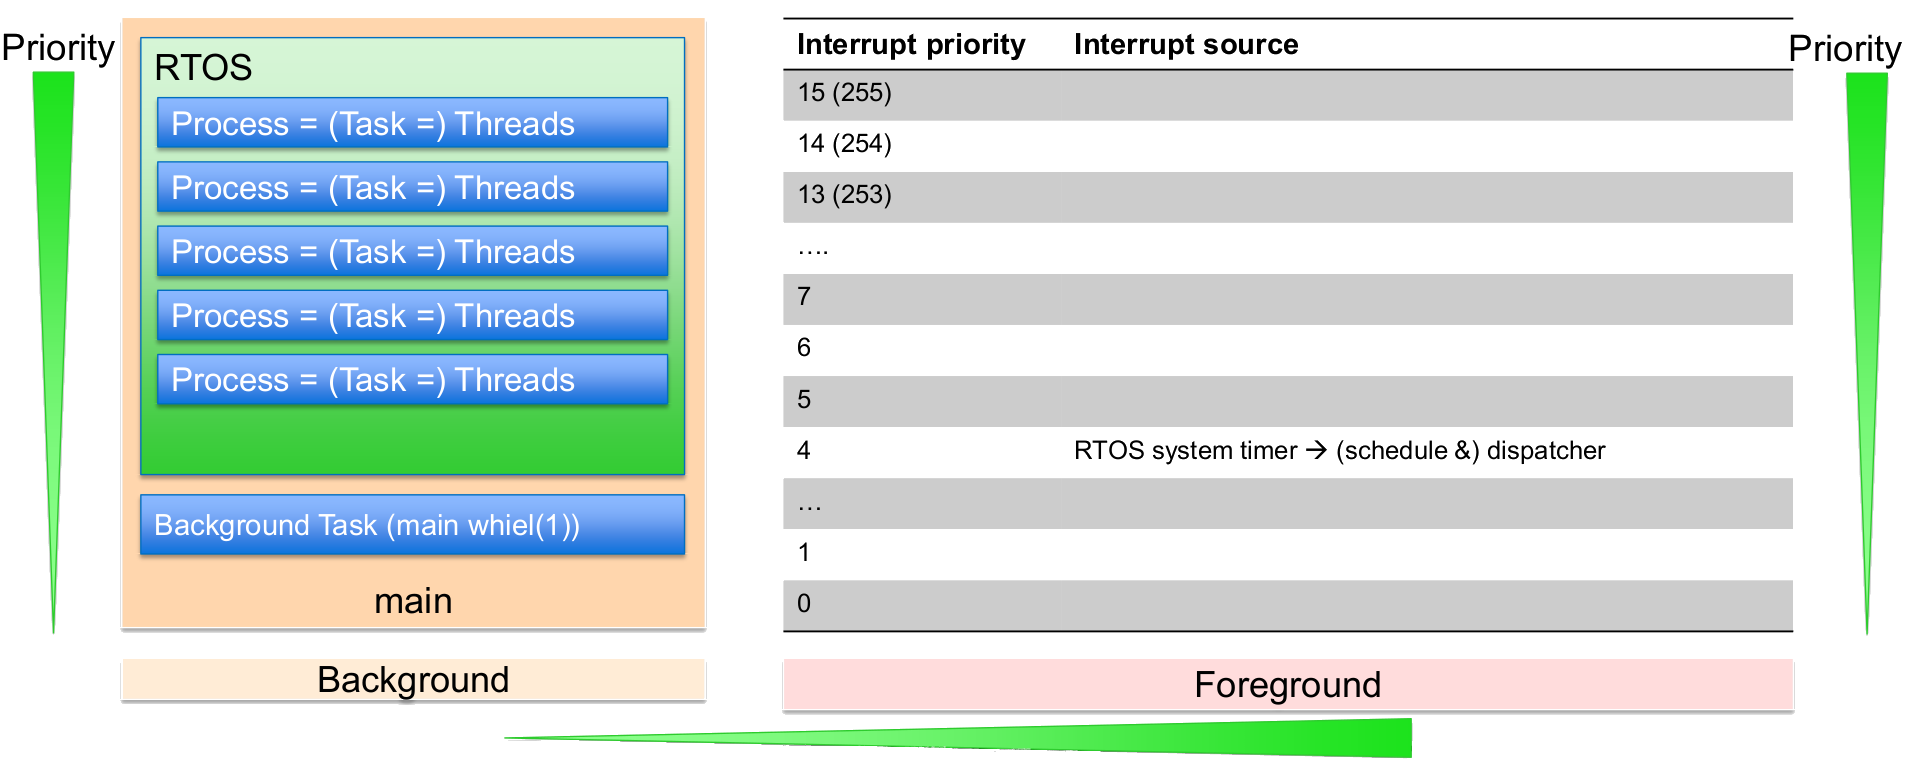
\includegraphics[width=\textwidth]{images/DesignStrategy/prio_interrupts_rtos_handling.png}
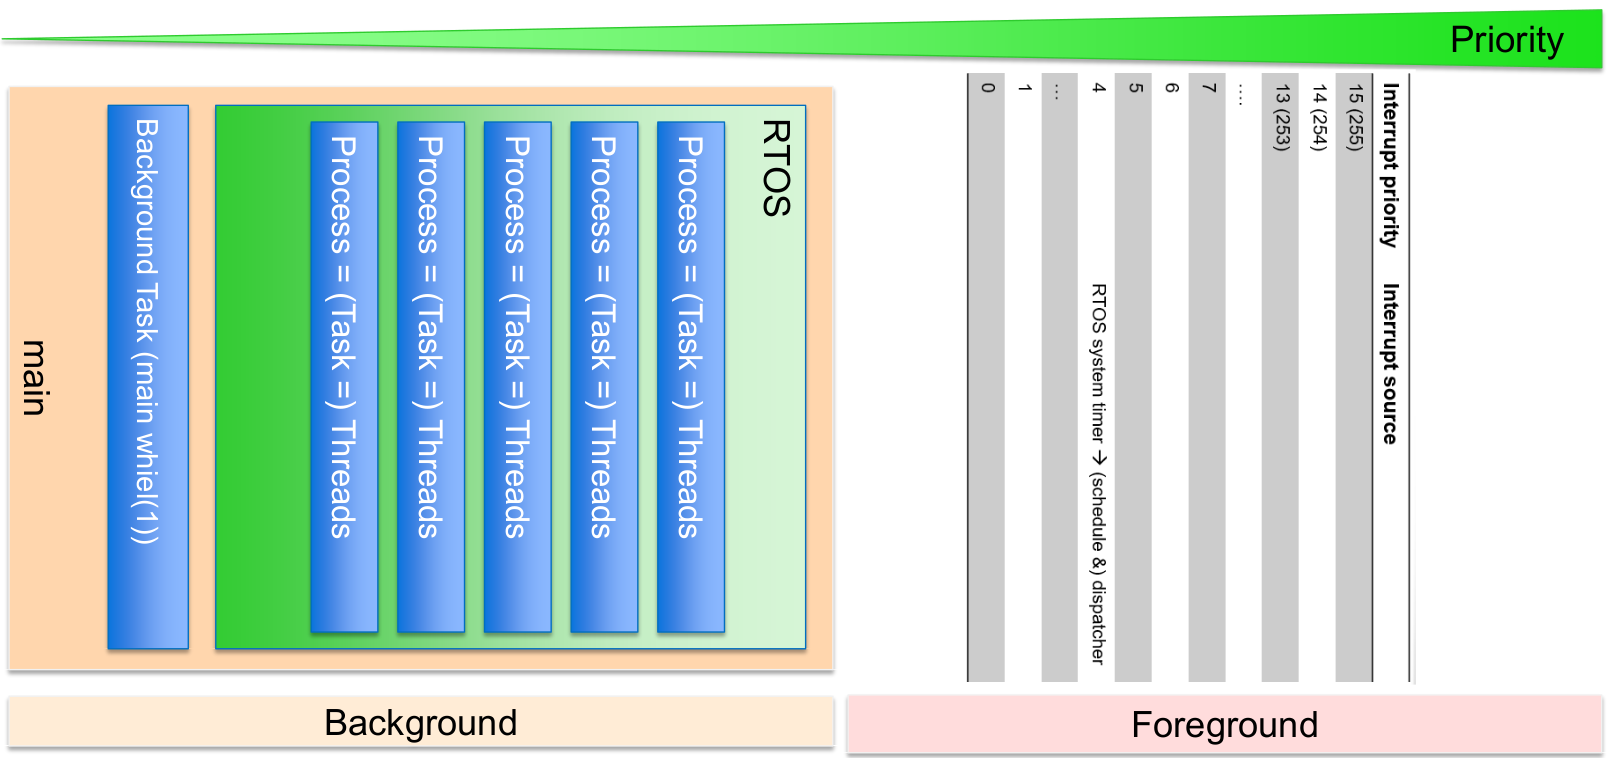
\includegraphics[width=\textwidth]{images/DesignStrategy/prio_interrupts_rtos_background.png}